\section{Training} \label{sec:res/training}

All classification models were trained on the cloud computing instance mentioned in section \ref{sec:impl/clf_models}. The time and computing resources required for training depended on label groups and the size of input tensors. However, results from averaging over these groups can be used to present an overall comparison between models. These results are given in table \ref{tab:res/training}.

\begin{table}[h!]
    \caption{Average time and epochs elapsed during training for all model architectures.}
    \makebox[\textwidth][c]{
        \begin{tabular}{l||ccccc}
            \diagbox{Average metrics}{Model}       & \acrshort{mlp}     & \acrshort{fcn}     & \acrshort{mcdcnn} & \acrshort{resnet11} & \acrshort{resnet18}  \\ 
            \hhline{=::=====}
            Epochs until best result    & 711     & 555     & 150    & 262      & 304       \\
            Training time per epoch   & 0.5s    & 5.5s    & 1.7s   & 7.9s     & 42s       \\
            Total training time       & 11m 52s & 50m 52s & 4m 16s & 41m 11s  & 3h 33m   
        \end{tabular}
    }
    \label{tab:res/training}
\end{table}
\FloatBarrier

\subsection{History}

The following plots present the history of training loss and accuracy for the two best \acrshort{fs} models, \acrshort{fcn} and \acrshort{resnet11}. Training loss was captured by logging the cross-entropy loss used to train model parameters during backpropagation. Validation accuracy was calculated by running the model on a validation dataset for every epoch. It is a percentage measure of how many classes were predicted correctly from a given set of inputs.

% \subsection{\acrlong{mlp}}

% \begin{figure}[h]
%     \centering
%     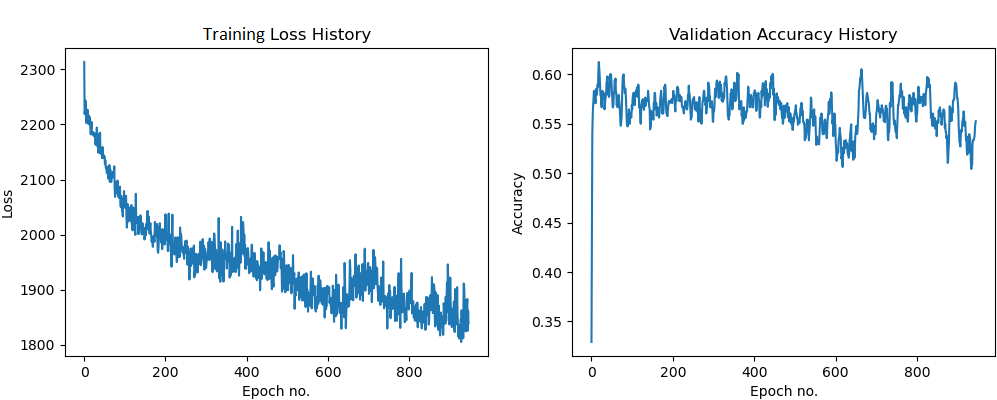
\includegraphics[width=\textwidth]{figures/res_tr_MLP_blevel.png}
%     \caption{Training loss and validation accuracy for \acrlong{mlp} during training. This particular example is from the binary level label group. Left graph shows the cross-entropy loss for every epoch. Right graph shows classification accuracy on the validation dataset for every epoch.}
%     \label{fig:res_tr_mlp}
% \end{figure}
% \FloatBarrier

\subsubsection{\acrlong{fcn}}

\begin{figure}[h]
    \centering
    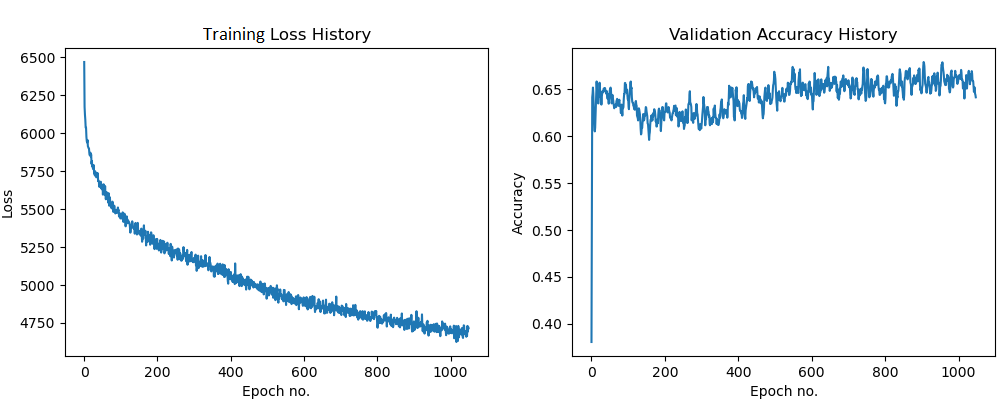
\includegraphics[width=\textwidth]{figures/res_tr_FCN_fstate.png}
    \caption{Training history for \acrlong{fcn} on the \acrshort{fs} label group. Left graph shows the cross-entropy loss for every epoch. Right graph shows classification accuracy on the validation dataset for every epoch.}
    \label{fig:res_tr_fcn}
\end{figure}
\FloatBarrier

% \newpage
% \subsection{\acrlong{mcdcnn}}

% \begin{figure}[h]
%     \centering
%     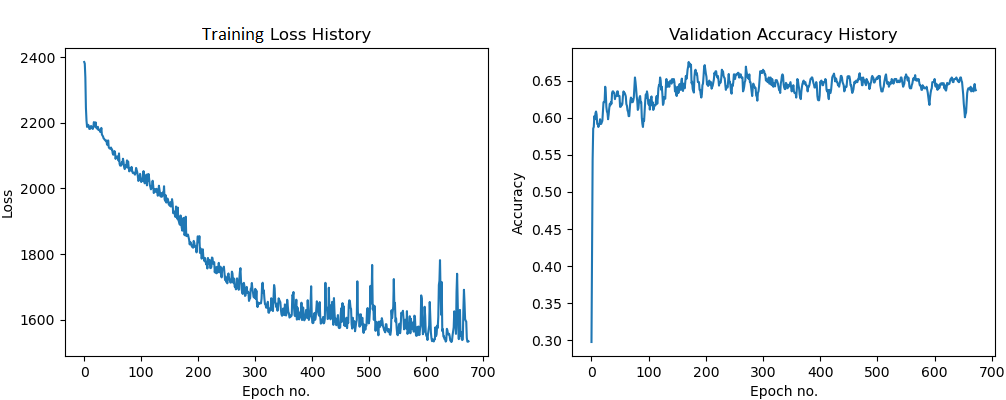
\includegraphics[width=\textwidth]{figures/res_tr_MCDCNN_blevel.png}
%     \caption{Training history for \acrlong{mcdcnn}. This particular example is from the binary level label group. See figure \ref{fig:res_tr_mlp} for plot descriptions.}
%     \label{fig:res_tr_mcdcnn}
% \end{figure}
% \FloatBarrier

\subsubsection{\acrlong{resnet11}}

\begin{figure}[h]
    \centering
    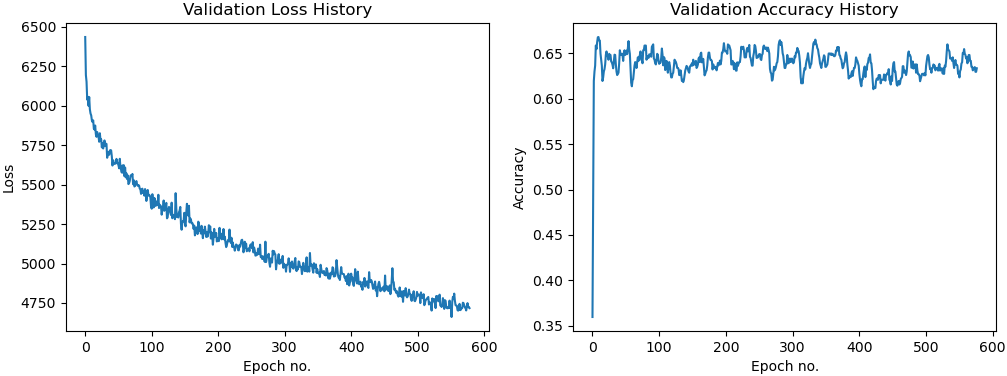
\includegraphics[width=\textwidth]{figures/res_tr_ResNet11_state.png}
    \caption{Training history for \acrlong{resnet11}on the \acrshort{fs} label group. See figure \ref{fig:res_tr_fcn} for plot description.}
    \label{fig:res_tr_resnet11}
\end{figure}
\FloatBarrier

% \newpage
% \subsection{\acrlong{resnet18}}

% \begin{figure}[h]
%     \centering
%     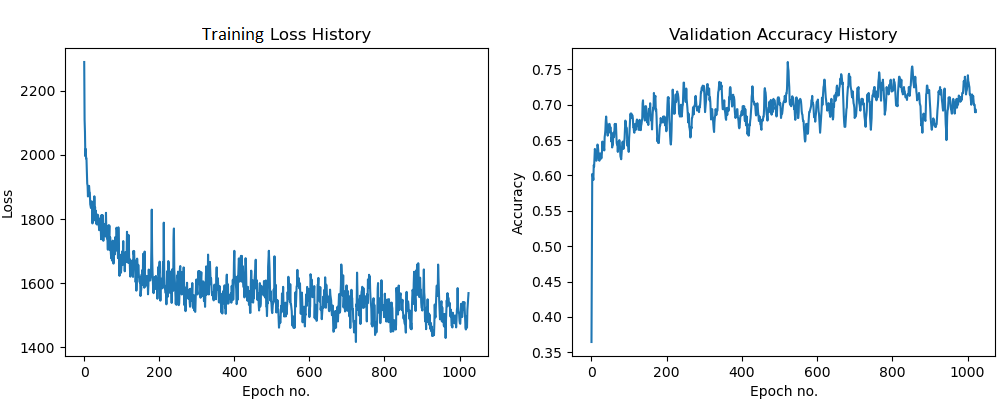
\includegraphics[width=\textwidth]{figures/res_ResNet18_blevel.png}
%     \caption{Training history for \acrlong{resnet18}. This particular example is from the binary level label group. See figure \ref{fig:res_tr_mlp} for plot descriptions.}
%     \label{fig:res_tr_resnet18}
% \end{figure}
% \FloatBarrier
\newpage
